\documentclass{article}

% if you need to pass options to natbib, use, e.g.:
%     \PassOptionsToPackage{numbers, compress}{natbib}
% before loading neurips_2018

% ready for submission
% \usepackage{neurips_2018}

% to compile a preprint version, e.g., for submission to arXiv, add add the
% [preprint] option:
%     \usepackage[preprint]{neurips_2018}

% to compile a camera-ready version, add the [final] option, e.g.:
     \usepackage[final]{nips_2018}

% to avoid loading the natbib package, add option nonatbib:
%     \usepackage[nonatbib]{neurips_2018}

\usepackage[utf8]{inputenc} % allow utf-8 input
\usepackage[T1]{fontenc}    % use 8-bit T1 fonts
\usepackage{hyperref}       % hyperlinks
\usepackage{url}            % simple URL typesetting
\usepackage{booktabs}       % professional-quality tables
\usepackage{amsfonts}       % blackboard math symbols
\usepackage{nicefrac}       % compact symbols for 1/2, etc.
\usepackage{microtype}      % microtypography
\usepackage{graphicx}
\usepackage{subcaption}
\usepackage{amsmath}

\graphicspath{ {imgs/} }

\title{CS 7180 Final Report}

% The \author macro works with any number of authors. There are two commands
% used to separate the names and addresses of multiple authors: \And and \AND.
%
% Using \And between authors leaves it to LaTeX to determine where to break the
% lines. Using \AND forces a line break at that point. So, if LaTeX puts 3 of 4
% authors names on the first line, and the last on the second line, try using
% \AND instead of \And before the third author name.

\author{%
  Nalin Gupta \\
  \texttt{NUID: 001497315} \\
  \And
  Christopher Botica\\
  \texttt{NUID: 001726854} \\
  \And
  Tyler Brown\\
  \texttt{NUID: 001684955} \\
  % Coauthor \\
  % Affiliation \\
  % Address \\
  % \texttt{email} \\
  % \AND
  % Coauthor \\
  % Affiliation \\
  % Address \\
  % \texttt{email} \\
  % \And
  % Coauthor \\
  % Affiliation \\
  % Address \\
  % \texttt{email} \\
  % \And
  % Coauthor \\
  % Affiliation \\
  % Address \\
  % \texttt{email} \\
}

\begin{document}
% \nipsfinalcopy is no longer used

\maketitle

\section{Introduction}

Images taken in low-light conditions are often too dark, noisy, and
distorted to be used in industrial purposes. We propose a deep-learning
model that processes low-light images to improve image brightness and
increase their overall quality. The problem with imaging in low-light
conditions is challenging due to low-photon count and low
Signal-to-Noise (SNR) ratio. These yield very dark and noisy images. The
most common technique to overcome this problem is long exposure shot.
However, this method yields blurry images with the slightest camera shake
or object motion\cite{chen2018learning}. Common post-processing
techniques brighten the image at the expense of image quality. Being able to
``see in the dark'' provides a number of real-world benefits such as
photography, computer vision, and social networking.

\section{Related Work}

In the past, the problem of enhancing low light images has been tackled via
noise reduction. This noise becomes dominant especially in low-light images
due to low SNR. Remez et. al. proposed a deep CNN for noise reduction under
the assumption that this low-light noise belongs to a Poisson
distribution \cite{remez2017deep}.  They used images from ImageNet
\cite{imagenet_cvpr09} as their ground truth data
and added synthetic Poisson noise to simulate corrupted images. Even though
their model outperform the state-of-the art de-noiser ``BM3D'', it does not
scale well to real world images, due to their underlying assumptions.... which ones...................??????????????????????????...
Furthermore, their model only denoises images but does not brighten them.
Motivated by these downfalls, Chen et. al., proposed an end-to-end CNN,
``See-in-the-Dark'' (SID), which brightens extremely low light images and
removes noise without making any underlying assumptions
\cite{chen2018learning}. However these advances come with the added expense
of collecting large amounts of low
light and bright light images. In the absence of a true vs noisy image
dataset, the team captured scenes using various exposure times to generate
true (bright light) and corrupted (low light) image pairs called
``See-in-the-Dark Dataset'' (SID Dataset
\footnote{https://github.com/cchen156/Learning-to-See-in-the-Dark}). Furthermore,
their model is camera specific and not easily generalizable.\newline

We propose a transferable CNN for image brightening and denoising. Instead
of training our model on actual true (bright light) and corrupted
(low light) image pairs, we use images from the publicly available
RAISE raw images dataset \cite{Dang-Nguyen:2015:RRI:2713168.2713194}. We
use the RAISE raw images dataset as our true images and corrupt these by
simulating low-light conditions for use in our model. We train our CNN on
this synthetic
data to obtain our initial model parameters. A small fraction of the real
images paired from the SID dataset is then used in our transfer learning
\cite{Goodfellow-et-al-2016} approach to update our model parameters.
These model parameters are updated for the particular camera used in the
SID dataset. We then use this model to test on the SID Dataset. In
addition, we aim to test various transfer learning approaches, such as the
traditional transfer learning and zero shot learning \cite{larochelle2008, NIPS2009_3650,socher2013zeroshot}. \newline

The novelty of our approach stems from the idea of ``more for less''. Our
model drastically reduces the overhead costs of data collection by
synthesizing readily available training data (RAISE raw images dataset).
This is
particularly beneficial in domains where collecting images pairs is
expensive/time consuming.

\section{Methods}

!!!... Say something like our flowchart: 
Simulate low light images -> then build deep cnn model --> then transfer learn to SID data .........


\subsection{Low Light Simulation}

We plan to use the RAISE raw images dataset which includes 6,000 high
definition images taken by professional photographers.

As illustrated in Figure 1, the traditional pipeline takes a corrupted image, and applies the following sequence of modules: Reduce Black Level, Denoising, White Balance, and Gamma Correction. The Black Level refers to refers to the level of brightness at the darkest parts of the image, and is reduced by subtracting the minimum pixel value. Denoising is reduced using common algorithms such as BM3D. White Balance refers to the color balance in the image (i.e., white should be true white) and is corrected by re-balancing the intensities of each color RGB. Finally, Gamma Correction controls the overall brightness of the image. We synthetically generate corrupted images by applying the reverse of this pipeline. Gamma Distortion: decrease the brightness of the image, White Imbalance: skew the color-space by multiplying each level of RGB by a random weight, Poisson Noise: add Poisson noise to the image, Black Level: add a negative bias to the pixel values (i.e., random black level). 

\begin{figure}[ht]
  \centering
  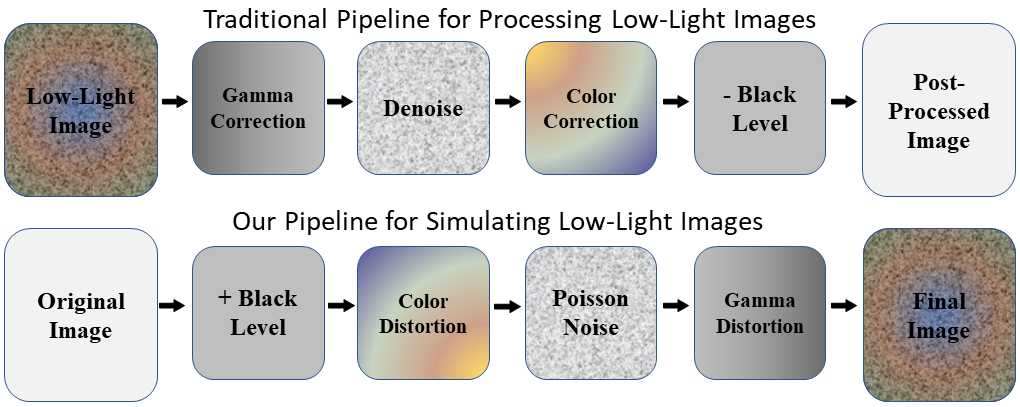
\includegraphics[scale=0.35]{simulation_flowchart}
  \caption{Top: Traditional Pipeline for processing low-light images. Bottom: Our  pipeline to simulate low-light images based on the traditional, only in reverse.}
\end{figure}

We simulate our low light images by successively applying gamma distortion, white imbalance, Poisson noise, and black level to a normal lighted. An example of two of such images is represented in Figure 3. 

For a given bright image, \(B\), a matrix of size \(m\)x\(n\)x3, we want to simulate a low-light image \(D\), or the same. We define gamma distortion as follows:
\[   D = {B}^{1/\gamma}, \] 
where \(\gamma\) controls the brightness of the image and the exponentiation is computed element-wise.

Furthermore, for the three channels of \(B\), namely \(B_{R}\), \(B_{G}\), and \(B_{B}\), and the three channels of \(D\), namely \(D_{R}\), \(D_{G}\), and \(D_{B}\), respectively, we define color distortion as follows:
\[ D_{R} = w_{R}*B_{R},\]
\[ D_{G} = w_{G}*B_{G},\]
\[ D_{B} = w_{B}*B_{B},\]
where \(w_{R}, w_{G}, w_{B}\) are small weights that distort the color space.  

We define the black level as follows: 
\[  D = max(B-bl,0), \]
where \(bl\) represents the amount of black level added to the image. Note that the closer the pixel values are to 0, the darker they are. The maximum of \(B - bl\) and 0 is taken so that no pixels are negative. \newline

Finally, we add Poison noise. Since this outputs values between \([0, 1]\), we first scale our image, apply Poison, and then re-scale as follows:
\[  D/255 = Poisson(B/255). \]


\begin{figure}[ht]
  \centering
  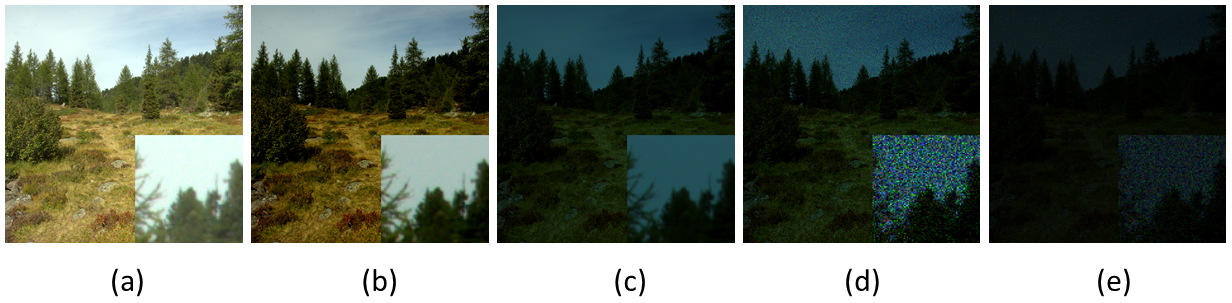
\includegraphics[scale=0.3]{simulation_all}
  \caption{Simulating low-light image via our pipeline: (a)..(b)...(c)...}
\end{figure}


Our initial approach to creating simulated low light images was to randomly select values for \(\gamma, w_{R}, w_{G}, w_{B},\) and \(bl\) was to choose these randomly and validate them by visualizing the distorted image. However, this process is not good enough to yield accurate results. The purpose of the simulation step is to simulate low light images the best we can, in order to then provide a well-trained model for transfer. Therefore, we assume values for these hyper-parameters for natural low-light images belong to certain distributions. In the next step, we aim to approximate these distributions.  \newline

Let \(b_{i,j,k}\) be a pixel value from \(B\) and \(d_{i,j,k}\) be a pixel value from \(D\). We approximate \(\gamma\) finding the value such, when gamma-distortion is applied to the bright image, the average pixel value equals that to the darker image:

\[  \frac{1}{3mn}\sum_{i,j,k}b_{i,j,k}^
{1/\gamma} = \frac{1}{3mn}\sum_{i,j,k}d_{i,j,k}\] 

Similarly, for a given pair \(B\) and \(D\), we find the optimal values for \(w_{R}, w_{G}, w_{B},\) and \(bl\), such that, after applying color-distortion, and adding black-level, respectively, the average pixel value for \(B\) equals that of \(D\). \newline

We repeat this process for 200 random pairs \(B\) and \(D\) from SID and compute the distribution for each value of \(\gamma, w_{R}, w_{G}, w_{B},\) and \(bl\). These distributions are exemplified in Figure 4. Our assumption is that, by sampling these values from their respective distribution, we can create more accurate low-light images. We find these distributions by computing
the Kernel Density Estimation (KDE) and then randomly sample. 

\begin{figure}[ht]
  \centering
  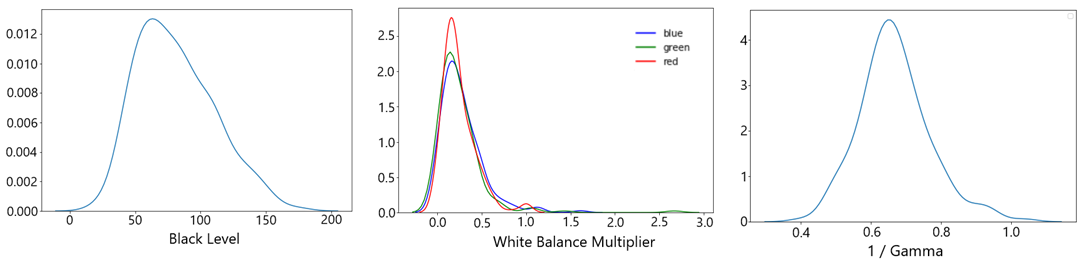
\includegraphics[scale=0.4]{Distributions}
  \caption{Distributions for (a) gamma, (b) RGB weights, and (c) black level.}
  \label{fig:train2}
\end{figure}




\subsection{Model}

Our model is .....This is highlighted in our model framework in Figure XX. 

\begin{figure}[ht]
  \centering
  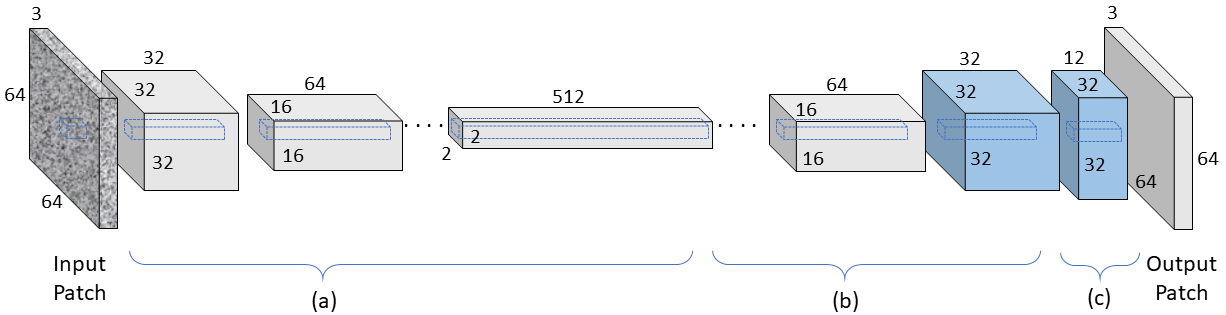
\includegraphics[scale=0.36]{model}
  \caption{Our proposed mode..add more!!!!!!!!!!l framework}
\end{figure}

More About Our model
More About Our Model
More About Our model.....
More About Our model
More About Our Model
More About Our model.....More About Our model
More About Our Model
More About Our model.....
More About Our model
More About Our Model
More About Our model.....


\subsection{Model Implementation}

We took inspiration from the SID model and wrote our own model which
had similar functionality. The SID model is mostly written in a higher
level Tensorflow contribution module called ``slim''. The ``slim''
contribution module does not appear to have any documentation and requires
one to read the module code embedded within Tensorflow. We initially tried
writing a model in parallel using Keras but found that moving from Keras
objects back down to lower level Tensorflow for some blocks within
forward propagation to not be documented well. We then rewrote the
Chen et. al. \cite{chen2018learning} model using only low level Tensorflow
code. This approach has the disadvantage of requiring the dimensions of
all weight matrices to be specified and initialized in a separate function
we called 'initialize\_parameters()'. \newline

These efforts allowed us to understand the dimensionality of both models at
each of the 10 blocks within their forward propagation. We used these
models to experiment with pooling window size, and stride
length for the convolutional layers. We also added up
to three additional blocks with different parameters in an attempt to
get the output dimensions to match the dimensionality of our input
image. \newline

We also tried using the CIFAR10 and ImageNet datasets as input. The primary
issue when replicating their model was related to dimensionality. The RGB
images in CIFAR10 and ImageNet have $m \times n \times 3$ dimensions.
However, the SID model takes as input Raw images which have
$m \times n \times 4$ dimensions. We were able to confirm that output
dimensions from Chen et. al. \cite{chen2018learning} follow the pattern
$2m \times 2n \times 3$ irrespective of the image size or type used. During
our experiment, we focused our debugging efforts on understanding whether
the dimensionality of a raw image as an input generated incompatible
dimensions with the target vector after model output. This error resulted
in our replicated model not being able to compute the cost function.\newline

Currently, we are working with raw images as input which have been corrupted
using our low light simulation; mentioned in Section 3.4. The results
for our model are shown in Section 4.3. At this point, we have not been
able to use RGB images, having $m \times n \times 3$ dimensions, to work
with our model. It is important for us to develop this
capability in order to qualitatively verify that we are correctly augmenting
image data. We are unable to view simulated images in raw format because
it requires us to know proprietary information about how a camera
generated an image. In order to generate output for this milestone, we
modified images from Chen et. al. \cite{chen2018learning}, such that

\begin{align*}
  X &= g(y_{train})\\
  Y &= y_{train}
\end{align*}

where function $g$ is an application of artificial noise to a clean
image in $y_{train}$ which is then trained against a corresponding
image where $g$ has not been applied.

(At some point mention CIFAR10 \cite{cifar10} and ImageNet
\cite{imagenet_cvpr09})  

\section{Experiment}

Stuff About Our experiment
Results.. just like the slides

\section{Discussion}

Currently, we are simulating low light images using (Section 3.4) using
raw images from the SID dataset. A drawback of this approach is that we
can modify the pixels of the image to simulate low light but we cannot
view these modifications as a RGB image. Our proposed next step is to modify
our model is so it is compatible with RGB images as input. We have identified
blocks within the model which most likely need to be changed. After
updating our model to accept RGB input, we will be implementing transfer
learning to obtain the final result. 

.........Discussion stuff from slides
+ path forward (what needs to be done next).
....


\bibliographystyle{unsrt}
\bibliography{references}

\end{document}
